
\documentclass{article}

\usepackage{amssymb}
\usepackage{amsmath}
\usepackage{pgfplots}
\usepackage{tikz}
\usepackage[top=0.9in, bottom=0.9in, left=1.5in, right=1.5in]{geometry}
\usepackage{xcolor}


\title{ECE421 Problem Set 2}
\author{Micol Altomare}
\date{} 

%%% BEGIN DOCUMENT
\begin{document}

\maketitle


\section{Problem 1}

Given data:

\begin{table}[htbp]
   \centering
   %\topcaption{Table captions are better up top} % requires the topcapt package
   \begin{tabular}{|c|c|} % Column formatting, @{} suppresses leading/trailing space
   \hline
      $x^{(i))}$    & $t^{(i)})$  \\ 
      \hline \hline
      1 & 6  \\
      2 & 4     \\
      3 & 2   \\
      4 & 1  \\
      5 & 3 \\
      6 & 6 \\
      7 & 10 \\
      \hline
   \end{tabular}
   \caption{Given data}
   \label{tab:booktabs}
\end{table}

\subsection{}

\begin{figure}[ht]
  \centering
  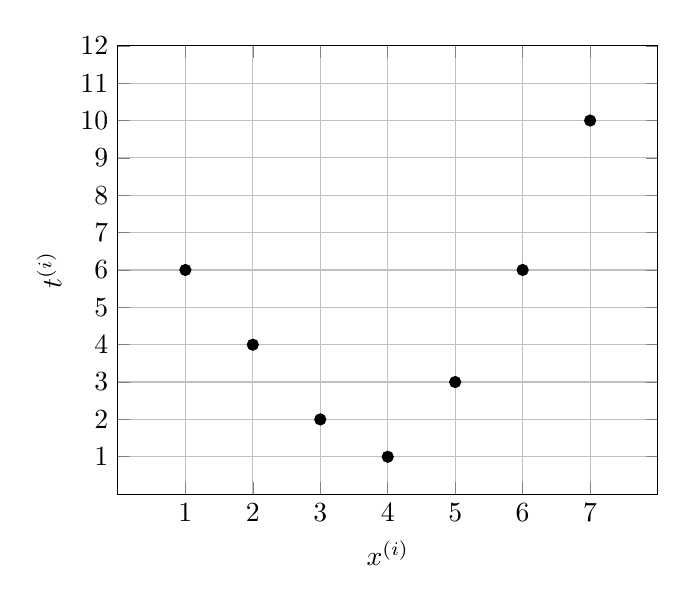
\begin{tikzpicture}
    \begin{axis}[
      xlabel={$x^{(i)}$},
      ylabel={$t^{(i)}$},
      xmin=0, xmax=8, % Adjust the axis limits as needed
      ymin=0, ymax=12,
      xtick={1,2,3,4,5,6,7},
      ytick={1,2,3,4,5,6,7,8,9,10,11,12},
      grid=both,
      mark=*, % Use asterisks as markers
      ]
      
      \addplot[only marks] table {
        1 6
        2 4
        3 2
        4 1
        5 3
        6 6
        7 10
      };
    \end{axis}
  \end{tikzpicture}
  \caption{Scatter plot of $x^{(i)}$ vs. $t^{(i)}$}
\end{figure}


\subsection{}

\begin{align*}
\mathcal{E} (w, b) &= \frac{1}{2N} \sum_{i = 1}^{N} (y^{(i)} - t^{(i)})^2 \\
&=  \frac{1}{2N} \sum_{i = 1}^{N} (wx^{(i)} - t^{(i)})^2 \\
&= \frac{1}{2N}  \sum_{i = 1}^{N}  \left[ (wx^{(i)})^2 + wx^{(i)}b -wx^{(i)} t^{(i)} + wx^{(i)}b + b^2 - bt^{(i)} - wx^{(i)}t^{(i)} - t^{(i)}b + (t^{(i)})^2 \right] \\
&= \frac{1}{2N}  \sum_{i = 1}^{N}  \left[ (w^2 x^{(i)})^2 + 2wx^{(i)} b - 2w x^{(i)} t^{(i)} - 2bt^{(i)} + b^2 + (t^{(i)})^2 \right] \\
&= \frac{1}{2N}  \sum_{i = 1}^{N} \left[ \textcolor{blue}{(x^{(i)})^2} w^2 + \textcolor{blue}{1}b^2 + \textcolor{blue}{2x^{(i)}}wb  \textcolor{blue}{-2t^{(i)}x^{(i)}}w \textcolor{blue}{ -2t^{(i)}}b + \textcolor{blue}{(t^{(i)})^2}	\right] \\
\implies A_i &= (x^{(i)})^2, B_i = 1, C_i = 2x^{(i)}, D_i = -2t^{(i)}x^{(i)}, E_i = -2t^{(i)}, F_i = (t^{(i)})^2 \\
\text{in} \; & \frac{1}{2N} \sum_{i = 1}^{N} A_i w^2 + B_i b^2 + C_i wb + D_i w + E_i b + F_i
\end{align*}

\subsection{}
\noindent The loss function is minimized when $\frac{\partial \mathcal{E}}{\partial w} = 0$ and $\frac{\partial \mathcal{E}}{\partial b} = 0$. Where $A = \sum_i A_i,$ etc....

\begin{align}
\frac{\partial \mathcal{E}}{\partial w} &=  \frac{1}{2N} \sum_{i = 1}^{N} 2wA_i + C_i b + D_i \\
&= 2wA + Cb + D = 0 \\
\implies w &= \frac{-Cb - D}{2A} \\
\frac{\partial{\mathcal{E}}}{\partial b} &=  \frac{1}{2N} \sum_{i = 1}^{N} 2 B_i b + C_i w + E_i \\
&= 2Bb + Cw + E = 0 \\
\implies b &= \frac{-Cw -E}{2B} \\
\implies w &= %%% solve
\end{align}


\subsection{}
By plugging in numerical values from the dataset D (Table 1), the values are found to be approximately:
\begin{align}
w&=
b &= 
\end{align}


\subsection{}
Using Excel's linear regression tool, it is found that $w$ = 2.1429 and $b$ = 0.6071.



\section{Problem 2}
\subsection{}
\subsection{}
\subsection{}
\subsection{}
\subsection{}


\section{Problem 3}
\subsection{}
\subsection{}
\subsection{}
\subsection{}
\subsection{}
\subsection{}



\end{document}